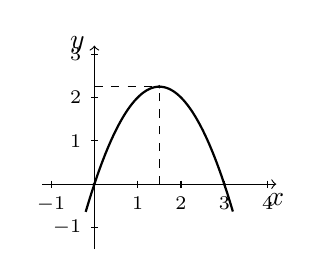
\begin{tikzpicture}[scale=0.55]
    \draw[->] (-1.2,0) -- (4.2,0) node[below] {$x$};
    \draw[->] (0,-1.5) -- (0,3.2) node[left] {$y$};
    \foreach \x in {-1,1,2,3,4}
        \draw (\x,0.08) -- (\x,-0.08) node[below] {\scriptsize $\x$};
    \foreach \y in {-1,1,2,3}
        \draw (0.08,\y) -- (-0.08,\y) node[left] {\scriptsize $\y$};
    \draw[smooth, samples=200, domain=-0.2:3.2, thick] plot (\x, {-(\x)*(\x-3)});
    \fill (0,0) circle (1.2pt);
    \fill (3,0) circle (1.2pt);
    \fill (1.5,2.25) circle (1.2pt);
    \draw[dashed] (1.5,0) -- (1.5,2.25);
    \draw[dashed] (0,2.25) -- (1.5,2.25);
\end{tikzpicture}
